\documentclass[12pt, a4paper]{report}
\usepackage[left=2cm, right=2cm, top=3cm, bottom=2cm]{geometry}
\usepackage{graphicx}
\usepackage{listings}
\usepackage{fancyhdr}
\usepackage{hyperref}
\usepackage{tcolorbox}
\usepackage{titlesec}
\usepackage{color}
\usepackage{xcolor}
\usepackage[utf8]{inputenc}
\usepackage[english]{babel}
\pagestyle{fancy}
\fancyhf{}
\rhead{Group Report}
\lhead{Collaborative Practical Project}
\rfoot{\thepage}
\definecolor{dkgreen}{rgb}{0,0.6,0}
\definecolor{gray}{rgb}{0.5,0.5,0.5}
\definecolor{mauve}{rgb}{0.58,0,0.82}

\begin{document}

\title{
\includegraphics[scale = .8]{UoM_Logo_Side_New.png}
\linebreak 
\linebreak 
\linebreak
\linebreak
\linebreak 
\textbf{CPS1010 - Collaborative Practical Project}\linebreak\linebreak
\large{B.Sc Computer Science}
\author{Chris Frendo\and Esther Spiteri\and Francesca Chircop \and Daniel Sumler\and Kelsey Marie Debono\and Tristan Oa Galea}}
\maketitle

\tableofcontents

\titleformat{\chapter}[display]
{\normalfont\huge\bfseries}{}{20pt}{\Huge}

% this alters "before" spacing (the second length argument) to 0
\titlespacing*{\chapter}{0pt}{-100pt}{40pt}

\chapter{Introduction}
The Agile Process is nowadays one of the most commonly used software development methodologies. It ensures a constant interaction between the client and user thus resulting in a higher end-product satisfaction. The aim of this assignment was to experience this process in a similar environment as to that in a workplace by carrying out sprints on a regular basis together with iterations. In addition weekly stand-up meetings were held between the team, throughout which scrum poker was used to establish user story points. This was done to ensure a better organization and order in which the tasks were executed. Throughout the assignment customer satisfaction was prioritised and adapting as a team to evolving user requirements was critical. 
\newline
\chapter{Project Process}

\section{First meeting}
A product inception meeting was set up and the project aim was clarified. The client's request was to have the team create an app together with a website in order to gather data from software developers through surveys. The users can answer questions through the app which the researcher publishes via the website. The researcher should then be able to view reports with data on his studies. These frontends communicate with a server which receives/sends data to/from a database. Following this meeting it was agreed that the work was to be split up as shown hereunder
\begin{itemize}
\item Chris Frendo and Daniel Sumler on the API
\item Esther Spiteri and Francesca Chircop on the APP
\item Kelsey Marie Debono and Tristan Oa Galea on the Website
\end{itemize}
Weekly standups were set and in each one every team member answered the following three questions:
\begin{enumerate}
    \item What has been carried out in the past week? 
    \item What are the current plans for the coming week?
    \item What problems were encountered? 
\end{enumerate} 
It was decided with the client that sprints were to each last two weeks and that we would meet at the end of each sprint. Iteration meetings between the team would take place once every two weeks to match with the client meetings. The team decided that it would be best if we were to meet at least once, ideally twice a week if possible, to have periods of working together in the same physical space. 

\newpage
\section{Iteration 0}
\normalsize
After the inception meeting with the customer the team had an idea of what technologies might be needed and an iteration 0 meeting was setup in order to discuss what technical infrastructure was to be used. During this iteration it was agreed that the team will use Trello as a Team Wall in order to be more organised by using checklists and due dates. Trello was also used for bug tracking and to keep a list of potential features that would be implemented if there was enough time. 
\begin{figure}[h]
\centering
\begin{center}
\fbox{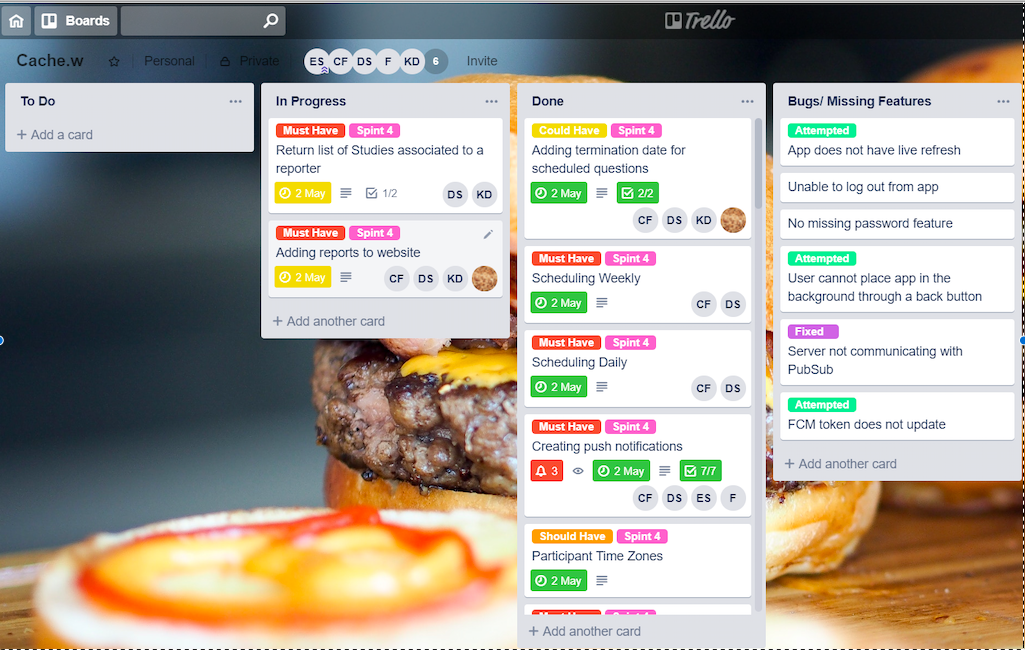
\includegraphics[scale=0.4]{images/trello1.png}}
\end {center}
\end{figure}
\newline
\normalsize
A github repository \textbf{\textit{[https://github.com/ChrisFrendo/Cachew]}} was used for version control. A Jenkins job was setup (configuration discussed later) to monitor builds. During Iteration 0 it was concluded as a team that as part of the process parameters of this project functionality would be given more importance over design and aesthetic since the latter required much more experience and keeping up with current trends. Every team member installed the respective tools and started doing research. 
\begin{itemize}
    \item API
    \begin{itemize}
        \item Node.js
        \item MongoDB
        \item Postman
    \end{itemize}
    \item APP
    \begin{itemize}
        \item Android SDK
        \item Ionic framework
        \item AngularJS
    \end{itemize}
    \item Website
    \begin{itemize}
        \item HTML, CSS and Javascript
        \item Bootstrap
    \end{itemize}
    
\end{itemize}
\section{Iteration 1}
\vspace*{5px}
\begin{tcolorbox}[width=\textwidth,colback={White},title={\textbf {Creation of Studies}},colbacktitle=grey,coltitle=black]
\underline{MoSCoW}: Must Have 
\hfill
\underline {Story points}: 40
\newline
\newline
 \blindtext \textbf{Description}
 \newline
In order to allow surveyors to create studies,
\newline
As a surveyor,\newline
I want to be able to create studies
\newline
\newline
 \textbf{Acceptance Criteria}
\newline
Given I am a surveyor,\newline
When I fill in the create study form,\newline
And it is filled in correctly,\newline
Then a new study should be created
\end{tcolorbox} 

\vspace*{20px}

\begin{tcolorbox}[width=\textwidth,colback={White},title={\textbf {Register}},colbacktitle=grey,coltitle=black]
\underline{MoSCoW}: Must Have 
\hfill
\underline {Story points}: 20
\newline
\newline
\blindtext \textbf{Description}
\newline
In order to allow users to use the website or application,
\newline
As a participant,
\newline
I want to be able to register for an account
\newline
\newline
 \textbf{Acceptance Criteria}
\newline
Given I am an unregistered user,\newline
When I fill in the registration form,\newline
And I fill it in correctly,\newline
Then I should be registered as a participant/surveyor
\end{tcolorbox} 

\subsubsection{Retrospectives}
\begin{itemize}
    \item Creation of studies took longer than expected as it was the first time the team was working together on these technologies.
    \item Specialized research of the task at hand was to be done in more detail. 
    \item Better time management was planned for the following iteration.
\end{itemize}

\section{Iteration 2}
\vspace*{5px}
\begin{tcolorbox}[width=\textwidth,colback={White},title={\textbf {Researchers only can login using website}},colbacktitle=grey,coltitle=black]
\underline{MoSCoW}: Must Have 
\hfill
\underline {Story points}: 8
\newline
\newline
\blindtext \textbf{Description}
\newline
In order to allow only researchers to access the website,\newline
As a participant, \newline
I should not be allowed to login \newline
\newline
 \textbf{Acceptance Criteria}
\newline
Given I am a registered researcher,\newline
When I try to login on the application, \newline
Then I should not be allowed, \newline
And shown an error message,\newline
\newline
Given I am a registered participant, \newline
When I try to login on the application, \newline
And I enter my login credentials correctly,\newline
Then I should be logged in 
\end{tcolorbox}  

\begin{tcolorbox}[width=\textwidth,colback={White},title={\textbf {Participants only can login using app}},colbacktitle=grey,coltitle=black]
\underline{MoSCoW}: Must Have 
\hfill
\underline {Story points}: 13
\newline
\newline
\blindtext \textbf{Description} \newline
In order to allow only participants to access the application, \newline
As a researcher, \newline
I should not be allowed to login \newline
\newline
 \textbf{Acceptance Criteria}
\newline
Given I am a registered participant,\newline
When I try to login on the website,\newline
Then I should not be allowed, \newline
And shown an error message, \newline
\newline
Given I am a registered researcher,\newline
When I try to login on the website,\newline
And I enter my login credentials correctly,\newline
Then I should be logged in
\end{tcolorbox}  

\vspace*{20px}

\begin{tcolorbox}[width=\textwidth,colback={White},title={\textbf {Delete Questions if Study POST fails}},colbacktitle=grey,coltitle=black]

\underline{MoSCoW}: Should Have  
\hfill
\underline {Story points}: 13
\newline
\newline
\blindtext \textbf{Description}\newline
In order to prevent having questions not linked to a study, \newline
When creating a study is not succesful, \newline
The website should send a delete request to delete the the submitted questions
\newline
\end{tcolorbox}  

\vspace*{20px}

\begin{tcolorbox}[width=\textwidth,colback={White},title={\textbf {Login Tokens}},colbacktitle=grey,coltitle=black]

\underline{MoSCoW}: Should Have  
\hfill
\underline {Story points}: 13
\newline
\newline
\blindtext \textbf{Description}\newline
In order to fetch only the logged in user's data,\newline
The system should store some sort of token or session id on the logged in user
\end{tcolorbox}  

\vspace*{20px}

\begin{tcolorbox}[width=\textwidth,colback={White},title={\textbf {Study subscriptions}},colbacktitle=grey,coltitle=black]
\underline{MoSCoW}: Must Have 
\hfill
\underline {Story points}: 8
\newline
\newline
\blindtext \textbf{Description}
\newline
In order to allow participants to subscribe to certain studies, \newline
As a participant, \newline
I should be allowed to choose which studies I want to subscribe to \newline
\newline
 \textbf{Acceptance Criteria}
\newline
Given I am a registered participant, \newline
When I click on a subscribe button on a particular study, \newline
Then I should be subscribed to that study 
\end{tcolorbox} 

\vspace*{20px}

\begin{tcolorbox}[width=\textwidth,colback={White},title={\textbf {Subscription Management}},colbacktitle=grey,coltitle=black]
\underline{MoSCoW}: Must Have 
\hfill
\underline {Story points}: 40
\newline
\newline
\blindtext \textbf{Description}
\newline
In order to allow only participant to manage their subscriptions,\newline
As a participant,\newline
I should have a page where I can view the studies I follow \newline
\newline
 \textbf{Acceptance Criteria}
 \newline
Given I am a registered participant, \newline
When I try access the supscribtions page on the app, \newline
Then I should see all of my subscribed studies, \newline
And there should be a way to unsubscribe from a particular study, 
\end{tcolorbox}  

\vspace*{20px}

\begin{tcolorbox}[width=\textwidth,colback={White},title={\textbf {Scheduling Questions}},colbacktitle=grey,coltitle=black]
\underline{MoSCoW}: Must Have 
\hfill
\underline {Story points}: 13
\newline
\newline
\blindtext \textbf{Description}
\newline
In order to schedule questions, \newline
As a researcher, \newline
I should have the option to specify the time to send particular questions of my study \newline
\newline
 \textbf{Acceptance Criteria}
 \newline
Given I am a registered researcher, \newline
When I create a study, \newline
Then I should be allowed to specify a time and date to ask each of my questions (in my own time zone) \newline
\end{tcolorbox}  

\vspace*{20px}

\begin{tcolorbox}[width=\textwidth,colback={White},title={\textbf {Study Search}},colbacktitle=grey,coltitle=black]
\underline{MoSCoW}: Would be nice to have
\hfill
\underline {Story points}: 40
\newline
\newline
\blindtext \textbf{Description}
\newline

In order to allow participants to search for studies, \newline
As a participant, \newline
I should have a page in the app where I can search for certain studies based on their genres, targets and title.\newline
\newline
 \textbf{Acceptance Criteria}
 \newline
Given I am a registered participant,\newline
When I am searching for study, \newline
Then I should be shown studies based on my search criteria. \newline
\end{tcolorbox}  

\vspace*{20px}

\begin{tcolorbox}[width=\textwidth,colback={White},title={\textbf {Study target demographics}},colbacktitle=grey,coltitle=black]
\underline{MoSCoW}: Must Have
\hfill
\underline {Story points}: 13
\newline
\newline
\blindtext \textbf{Description}
\newline
In order to allow researchers to select their target demographic for a particular study, \newline
As a researcher, \newline
I should be allowed to specify my targets based on their demographics (age, country, industry, job role, gender etc...) or specify that this is a generic study \newline \newline
 \textbf{Acceptance Criteria}
 \newline
Given I am a registered researcher, \newline
When I am creating a study, \newline
Then I should be given the option to specify my target demographic \newline
\end{tcolorbox}  

\subsubsection{Retrospectives}
\begin{itemize}
    \item Time management was observed to improve from the previous iteration.
    \item Scheduling of questions was not completed fully.
    \item In this iteration the team agreed on too many user stories due to lack of experience so in future meetings with the customer there were better discussions regarding workloads which also helped to manage customer expectations and prioritisation.
    \item During this iteration the team realised that it was important to think of future features that the user might want to implement in order to have the current features compatible with the future ones. This is why it was decided that project visibility was to be discussed with the client during following meetings.
\end{itemize}

\section{Iteration 3}
\vspace*{5px}

\begin{tcolorbox}[width=\textwidth,colback={White},title={\textbf {Targeted Study Search}},colbacktitle=grey,coltitle=black]
\underline{MoSCoW}: Should have
\hfill
\underline {Story points}: 20
\newline
\newline
\blindtext \textbf{Description}
\newline

In order to search for studies,\newline
As a user,\newline
I should see a list of studies which are targetted to my demographics\newline
\newline
 \textbf{Acceptance Criteria}
 \newline
Given I am a user,\newline
When I go on the new studies page,\newline
Then I should see only studies which are targetted to my profile
\newline
\newline
\underline{N.B.} API should have some sort of checking to only send studies which are targetted to the logged in user \newline
\end{tcolorbox}  

\vspace*{20px}

\begin{tcolorbox}[width=\textwidth,colback={White},title={\textbf {Study questions notification}},colbacktitle=grey,coltitle=black]
\underline{MoSCoW}: Would be nice to have
\hfill
\underline {Story points}: 40
\newline
\newline
\blindtext \textbf{Description}
\newline

In order to know when a question is available to answer,\newline
As a user,\newline
I should see the number of questions next to the study\newline
\newline
 \textbf{Acceptance Criteria}
 \newline
Given I am a user,\newline
When I subscribe to a study,\newline
Then I should see the number of questions available\newline
\end{tcolorbox}  

\vspace*{20px}

\begin{tcolorbox}[width=\textwidth,colback={White},title={\textbf {Flag to indicate scheduled questions}},colbacktitle=grey,coltitle=black]
\underline{MoSCoW}: Would be nice to have
\hfill
\underline {Story points}: 20
\newline
\newline
\blindtext \textbf{Description}
\newline

In order to know if a study has scheduled questions,\newline
As a user,\newline
I should see an icon next to my subscribed studies to indicate that this study has scheduled questions
\newline
\newline
 \textbf{Acceptance Criteria}
 \newline
Given I am a user,\newline
And I am subscribed to at least one study,\newline
When I open the dashboard page,\newline
Then I should see my list of subscribed studies,\newline
And next to each study which has scheduled questions there should be an icon to indicate this.
\newline\newline
\underline{N.B.} API needs to send a boolean for front end to interpret
\end{tcolorbox}  

\vspace*{20px}

\begin{tcolorbox}[width=\textwidth,colback={White},title={\textbf {Multiple Choice}},colbacktitle=grey,coltitle=black]
\underline{MoSCoW}: Must Have
\hfill
\underline {Story points}: 5
\newline
\newline
\blindtext \textbf{Description}
\newline

In order to allow researchers to ask a multiple choice question\newline
As a researcher,\newline
I should be allowed to input the different choices a user can choose in a single \newline
text box delimited by a new line character
\newline
\newline
 \textbf{Acceptance Criteria}
 \newline
Given I am a registered researcher,\newline
When I am creating a study,\newline
Then I should be given the option to ask a multiple choice question
\end{tcolorbox}  

\vspace*{20px}

\begin{tcolorbox}[width=\textwidth,colback={White},title={\textbf {Updating Scheduling UI}},colbacktitle=grey,coltitle=black]
\underline{MoSCoW}: Must Have
\hfill
\underline {Story points}: 20
\newline
\newline
\blindtext \textbf{Description}
\newline

In order to allow researchers to schedule different questions at different times,\newline
As a researcher,\newline
I should be allowed to specify my preferred scheduling times for different questions from a drop down menu. The options in this menu include: 'Just Once', 'Daily', 'Weekly', 'Monthly'.
\newline
\newline
 \textbf{Acceptance Criteria}
 \newline
Given I am a registered researcher,\newline
When I am creating a study,\newline
I should be able to schedule questions I create based on a date and a frequency preference
\end{tcolorbox}  

\vspace*{20px}

\begin{tcolorbox}[width=\textwidth,colback={White},title={\textbf {Updating Study Target Demographics UI}},colbacktitle=grey,coltitle=black]
\underline{MoSCoW}: Could Have
\hfill
\underline {Story points}: 8
\newline
\newline
\blindtext \textbf{Description}
\newline

In order to allow researchers to select their target demographic for a particular study,\newline
As a researcher,\newline
I should be allowed to specify my targets based on their demographics (age, country, industry, job role, gender etc...) or specify that this is a generic study, allowing the researcher to choose multiple targets
\newline
\newline
 \textbf{Acceptance Criteria}
 \newline
Given I am a registered researcher,\newline
When I am creating a study,\newline
Then I should be given the option to specify more than one target demographic 
\end{tcolorbox}  

\vspace*{20px}

\begin{tcolorbox}[width=\textwidth,colback={White},title={\textbf {Study page}},colbacktitle=grey,coltitle=black]
\underline{MoSCoW}: Must Have
\hfill
\underline {Story points}: 40
\newline
\newline
\blindtext \textbf{Description}
\newline

In order to answer questions,\newline
As a user,\newline
I should have a question page
\newline
\newline
 \textbf{Acceptance Criteria}
 \newline
Given I am a user,\newline
When a study has a question,\newline
Then I should be allowed to answer it through a question page
\end{tcolorbox}  

\subsubsection{Retrospectives}
\begin{itemize}
    \item Refresh issues were encountered in the app in order to update data when questions are completed or new questions are sent by the researcher. This was partially overcome via refresh on switching back to the subscribed study page. However, a solution for live refresh was not found. 
    \item Improvement in time management resulted in a better presentation of work during the iteration meeting. 
\end{itemize}

\newpage
\section{Iteration 4}
\vspace*{5px}

\begin{tcolorbox}[width=\textwidth,colback={White},title={\textbf {Adding Tests for API}},colbacktitle=grey,coltitle=black]
\underline{MoSCoW}: Should Have
\hfill
\underline {Story points}: 8
\newline
\newline
\blindtext \textbf{Description}
\newline
Add tests using postman to be used when building job in jenkins\newline
\end{tcolorbox}  

\vspace*{20px}

\begin{tcolorbox}[width=\textwidth,colback={White},title={\textbf {Scheduling Just Once}},colbacktitle=grey,coltitle=black]
\underline{MoSCoW}: Must Have
\hfill
\underline {Story points}: 20
\newline
\newline
\blindtext \textbf{Description}
\newline
In order for the app to show just once scheduled questions when their time comes,\newline
The server should check whether a question's time is within 5 mins of the current \newline \newline
\underline{N.B}: The Server should also take into account the timezones of both the researcher when creating the question and the user who is requesting the question.
\end{tcolorbox} 

\vspace*{20px}

\begin{tcolorbox}[width=\textwidth,colback={White},title={\textbf {Adding termination date for scheduled questions}},colbacktitle=grey,coltitle=black]
\underline{MoSCoW}: Could Have 
\hfill
\underline {Story points}: 20
\newline
\newline
\blindtext \textbf{Description}
\newline
In order to be able to input a termination date for a daily/weekly scheduled question, \newline
As a researcher, \newline
I should have an input field where I can enter the termination date for my question 
\newline
\newline
 \textbf{Acceptance Criteria}
 \newline
Given I am a logged in reseracher, \newline
When I am creating a new question for a study, \newline
And I selected a daily or weekly schedule, \newline
Then an input field should pop up where I can enter the termination date for my question 
\newline
\end{tcolorbox}  

\vspace*{20px}

\begin{tcolorbox}[width=\textwidth,colback={White},title={\textbf {Participant Time Zones}},colbacktitle=grey,coltitle=black]
\underline{MoSCoW}: Should Have
\hfill
\underline {Story points}: 13
\newline
\newline
\blindtext \textbf{Description}
\newline
In order to recieve questions at the correct time,\newline
The system should push questions to the participants according to their timezones
\newline
\end{tcolorbox}  

\vspace*{20px}

\begin{tcolorbox}[width=\textwidth,colback={White},title={\textbf {Scheduling Weekly}},colbacktitle=grey,coltitle=black]
\underline{MoSCoW}: Must Have
\hfill
\underline {Story points}: 40
\newline
\newline
\blindtext \textbf{Description}
\newline
In order for the app to show daily scheduled questions when their time comes,\newline
The server should check whether a question's scheduled time is within 5 mins of the current time
\newline
\newline
\underline{N.B}:  The Server should also take into account the timezones of both the researcher when creating the question and the user who is requesting the question.
\end{tcolorbox}  

\vspace*{20px}

\begin{tcolorbox}[width=\textwidth,colback={White},title={\textbf {Scheduling Daily}},colbacktitle=grey,coltitle=black]
\underline{MoSCoW}: Must Have
\hfill
\underline {Story points}: 40
\newline
\newline
\blindtext \textbf{Description}
\newline
In order for the app to show daily scheduled questions when their time comes,\newline
The server should check whether a question's scheduled time is within 5 mins of the current time
\newline
\newline
\underline{N.B}:  The Server should also take into account the timezones of both the researcher when creating the question and the user who is requesting the question.
\end{tcolorbox}  

\vspace*{20px}

\begin{tcolorbox}[width=\textwidth,colback={White},title={\textbf {Creating push notifications}},colbacktitle=grey,coltitle=black]
\underline{MoSCoW}: Must Have
\hfill
\underline {Story points}: 40
\newline
\newline
\blindtext \textbf{Description}
\newline
In order to be able to recieve push notifications when a question is availabe,
\newline
The app should be connected to fcm and send the server the fcm token.
\newline
\newline
The server should be connected to pubsub and fcm. The server should also create a topic for each study and subscribe participants on firebase through their fcm tokens to the studies which they subscribe to.
\newline
\newline
The server should also have a cron job running every minute to check for any due questions and send a push notification if it finds one.
\end{tcolorbox} 

\vspace*{20px}

\begin{tcolorbox}[width=\textwidth,colback={White},title={\textbf {Return list of Studies associated to a reporter}},colbacktitle=grey,coltitle=black]
\underline{MoSCoW}: Must Have
\hfill
\underline {Story points}: 20
\newline
\newline
\blindtext \textbf{Description}
\newline
In order to be able to select a study to view reports,
\newline
As a researcher,
\newline
I should have a dropdown list with the study titles that I created
\newline
\newline
 \textbf{Acceptance Criteria}
 \newline
Given I am a logged in researcher,
\newline
When I am on the reports page,
\newline
Then I should have a drop down list populated with my studies' titles.
\end{tcolorbox} 

\vspace*{20px}

\begin{tcolorbox}[width=\textwidth,colback={White},title={\textbf {Adding reports to website}},colbacktitle=grey,coltitle=black]
\underline{MoSCoW}: Must Have
\hfill
\underline {Story points}: 40
\newline
\newline
\blindtext \textbf{Description}
\newline
In order to be able to view reports for questions,
\newline
As a researcher,
\newline
I should have a page where I can view the reports in a graphical manner where appropriate
\newline
\newline
 \textbf{Acceptance Criteria}
 \newline
Given I am a logged in researcher,
\newline
When I want to view the reports for my studies,
\newline
Then I should have a page where I can access my studies and view reports for their questions.
\newline
\newline
\underline{N.B}:  The reports should have a live update feature and they should have buttons to change chart type. Client also said that if we want we can add export to CSV option.
\end{tcolorbox} 

\subsubsection{Retrospectives}
\begin{itemize}
    \item The work on time specifications was continued.
    For example an input field was added in order to be able to input a termination date for a scheduled question. In addition the time zones were also set for both the researcher and the user.
    \item Tests were added using postman to be used when building job in jenkins. 
    \item Everything was joined together and the last final touches were sorted and divided again between the contributors. 
    \item It was observed that things went more smoothly in this iteration since the members had a much better idea on the workload of each story and because the team was gaining experience working with the technologies.
\end{itemize}
\newpage
\section{Wire Frames}
\begin{figure} [h]
\centering
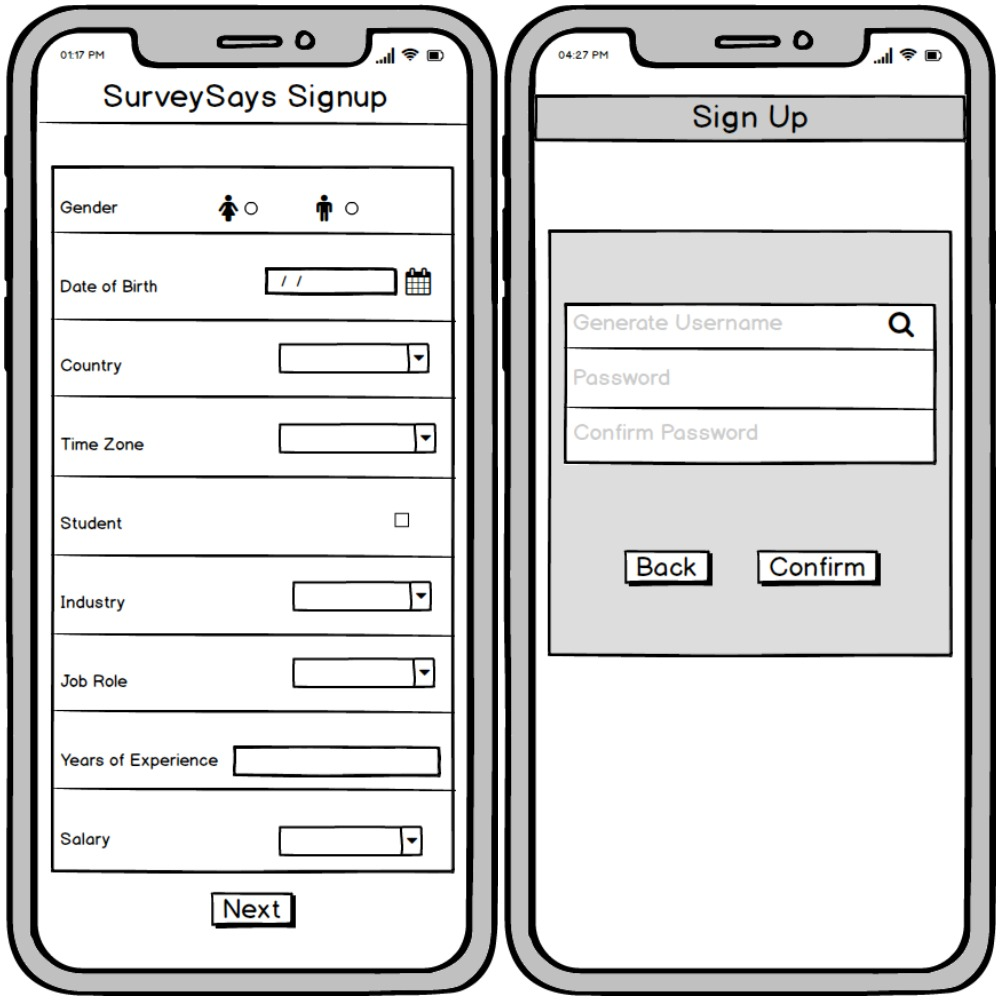
\includegraphics[scale=0.35]{images/pic1.jpeg}
\caption{\centering Sign up page including details page, username generator \& password setup}
\end{figure}
\begin{figure} [h]
\centering
\begin{center}
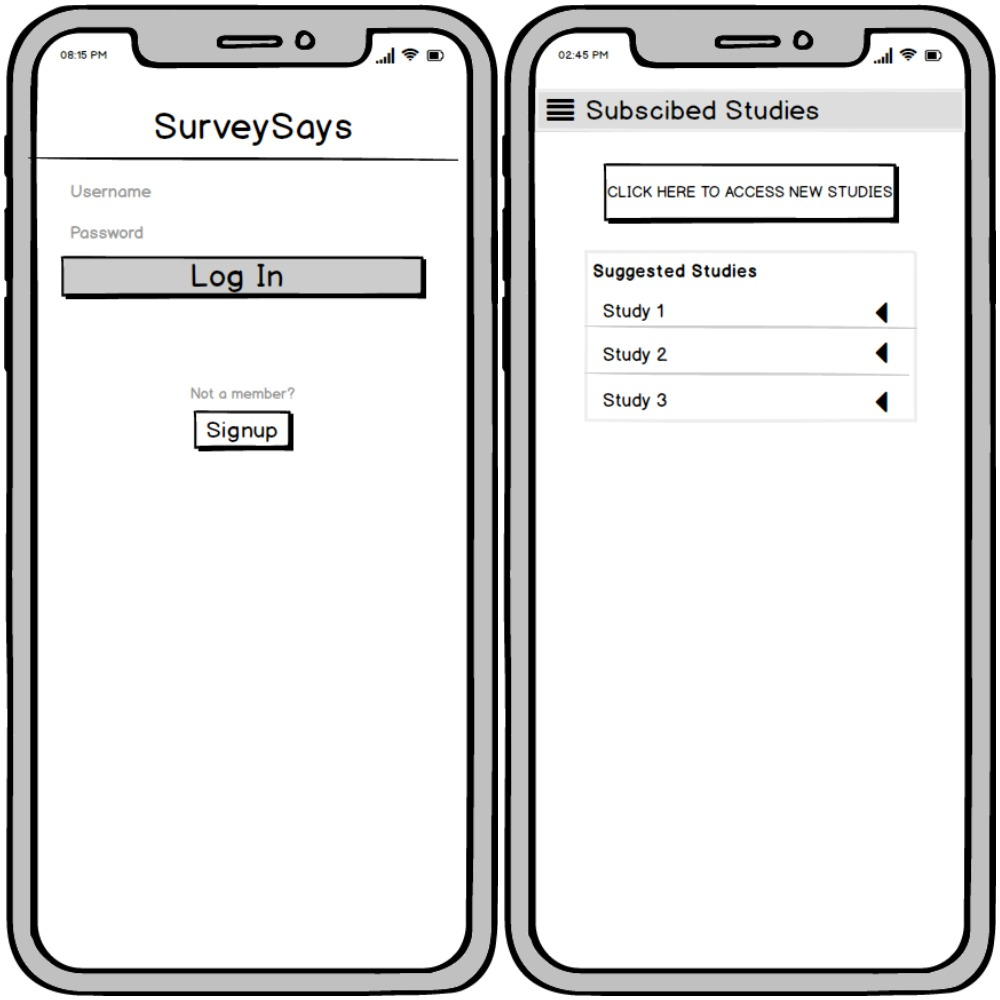
\includegraphics[scale=0.35]{images/pic2.jpg}
\end{center}
\caption{\centering Log in page including sign up button \& user dashboard page including suggested studies if no subscribed to studies}
\end{figure}
\begin{figure} [h]
\centering
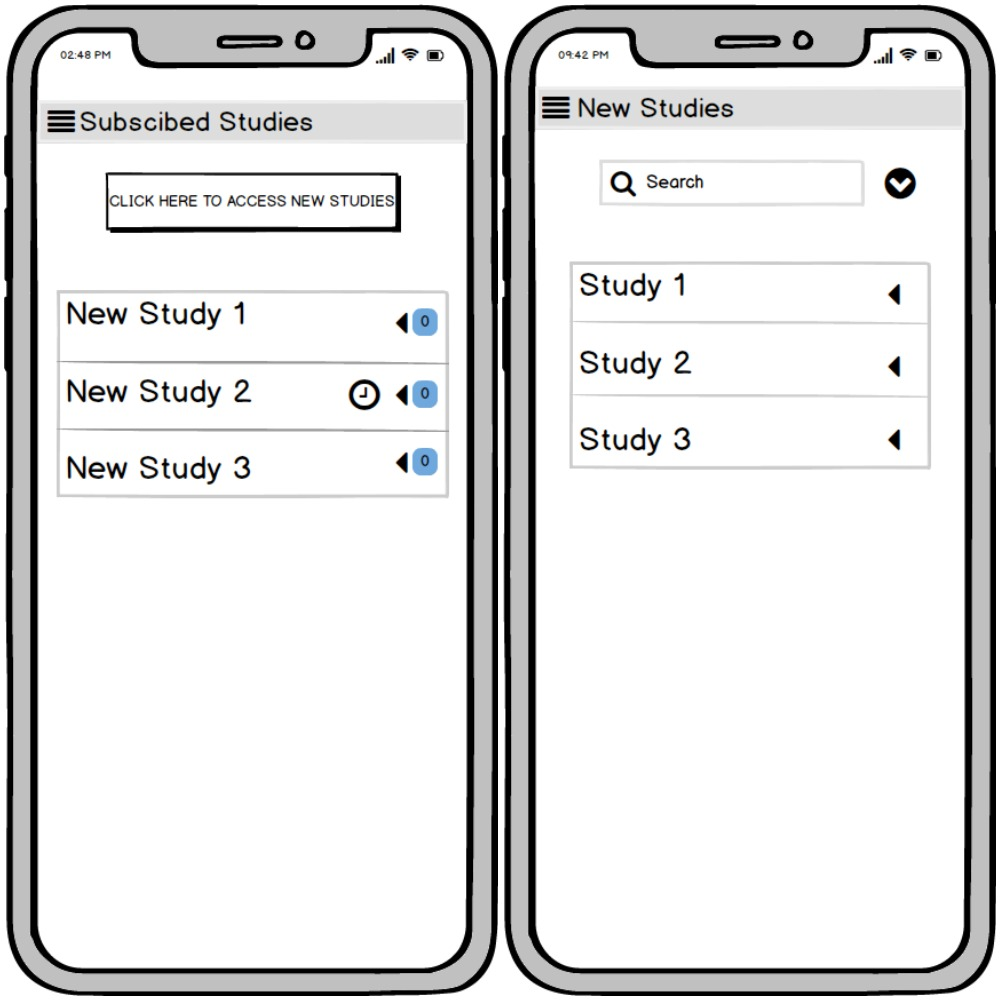
\includegraphics[scale=0.35]{images/pic4.jpg}
\caption{\centering Subscribed Studies page including a button to access more studies & New Studies page including a search box}
\end{figure}
\begin{figure} [h]
\centering
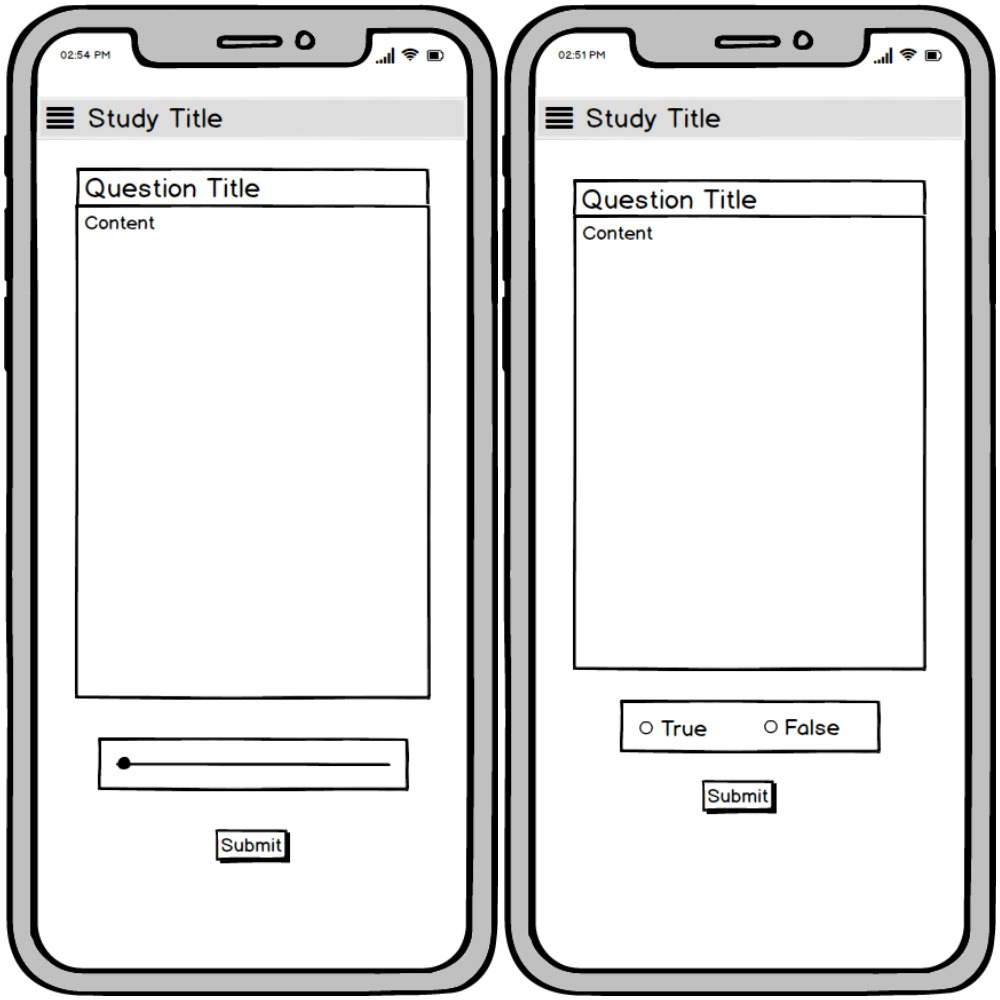
\includegraphics[scale=0.35]{images/pic3.jpg}
\caption{\centering Study pages including one with a slider (Rating question) and boolean type}
\end{figure}
\begin{figure} [h]
\centering
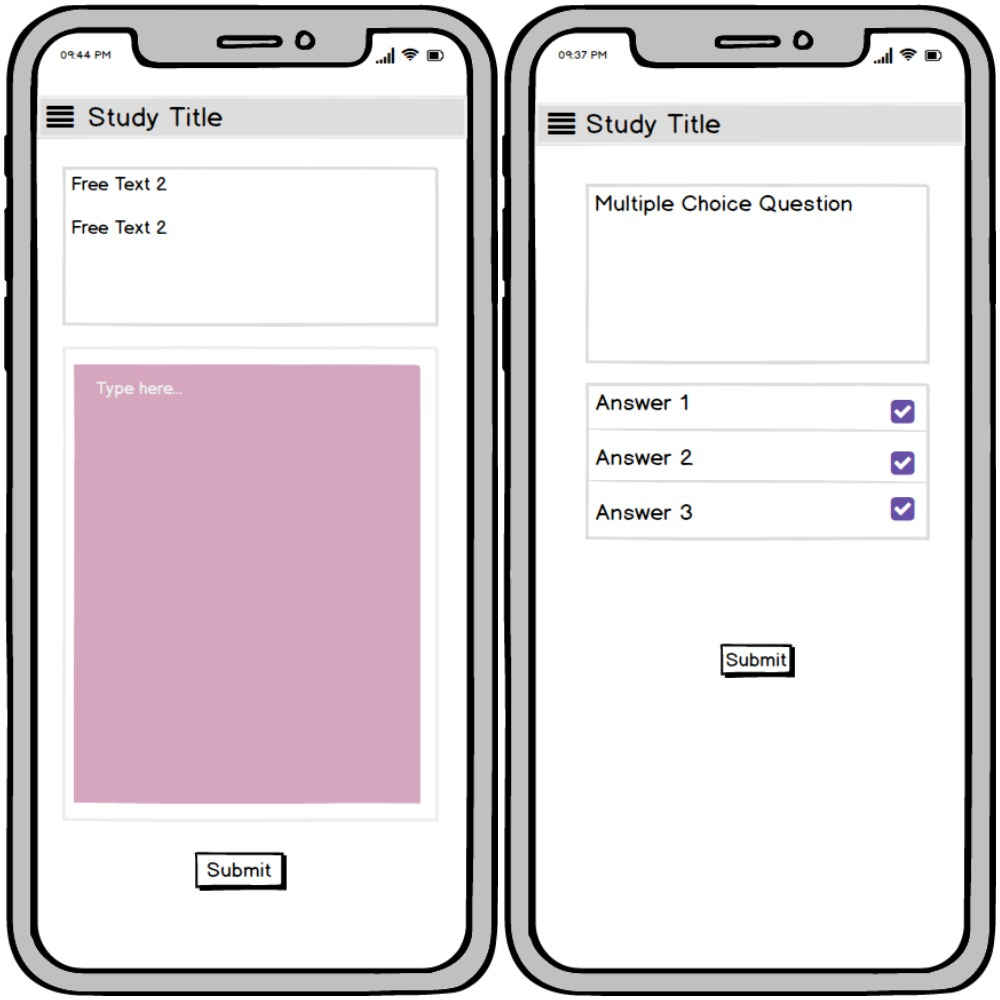
\includegraphics[scale=0.35]{images/pic5.jpg}
\caption{\centering Study pages including one with an open ended question and  multiple choice question}
\end{figure}

\clearpage


\newpage
\section{Improvements throughout the iterations}
\begin{enumerate}
    \item MoSCoW was introduced between the first and the second iteration. [However, for completeness, MoSCoW was also applied to the previous iterations.]
    \item From one iteration to the other, judgement of the user stories' workloads and priorities was improved. More consideration was being taken when assigning story points to the tasks in order to achieve more realistic time frames. 
    \item Co-ordination between the three teams in order to work simultaneously on the same task was improved throughout the allocated time for co-located work.
    \item Issues on Github were implemented for iteration 4 to better organise issues and enhancements between the collaborators.
\end{enumerate}

\section{Showcases}
\paragraph{\;\;\:}
\noindent
Showcases were carried out biweekly with the client. During these meetings the team would first show the customer the newly added functionalities from the previous iteration and then discuss the next set of features to be implemented in the following sprint. During these showcases the team would give a brief overview on how the particular feature was implemented without going into extra technical details unless the customer asks for it. 
\paragraph{\;\:\:}
\noindent
In all showcases the client was satisfied with the team's work and results especially in the last two iterations since the client could see the differences in the newly added features. After giving the customer a demo of the added functions and verifying that the client is satisfied with the product a release would be created on GitHub. This was done to ensure that there was a record for each showcase presented to the client, and it helped with sorting the time-line of all commits into versions. 

\newpage
\chapter{Jenkins configuration and instructions}

A Jenkins job called \textit{Cache.w} was created to keep track of git changes and keep the team informed if any builds failed. It was setup to poll every 15 minutes from the github repository's master branch and check if there had been any changes. If there were then it would create a build. When building it executes a shell script which uses \textit{newman} to run a custom postman test script. An snippet of a build's console output can be seen below. If the build fails due to a failing test or any other cause, Jenkins will send emails to all the team members.
\begin{figure} [h]
\centering
\fbox{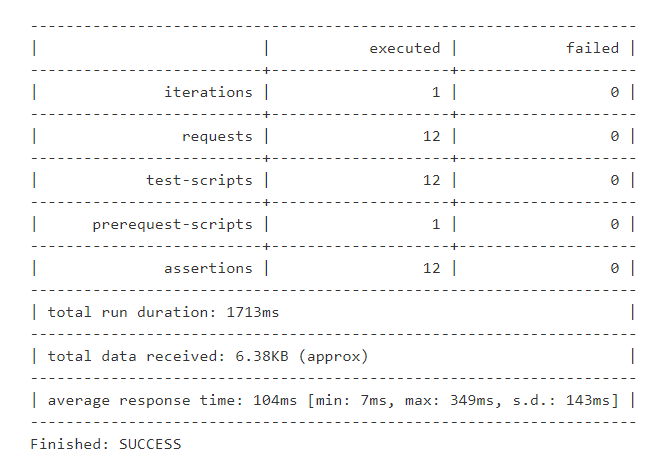
\includegraphics[scale=1]{images/Jenkins.png}}
\end{figure}
The project consists of three main parts as discussed before: Server, Website and Mobile App. Note that the app was not tested on an iPhone since there were problems when installing dependencies on the Mac machine so the instructions will be for android.
\begin{itemize}
\item Website
	\begin{itemize}
		\item When connected on the UoM network either through wifi or vpn simply enter the ip 10.60.10.66 in the address bar of your browser to access the website.
		\item Alternatively you can download the files from Jenkins and open the html files which can be found in the directory \textit{SurveySaysWebsite}.
	\end{itemize}
\item App
	\begin{itemize}
		\item The app is available on the Google Play store. Simply search Survey Says on the Play store or enter \textit{https://play.google.com/store/apps/details?id=com.cachew.surveySays}
		\item Alternatively you can download the files from Jenkins and run the application in an emulator on your machine. 
		\begin{enumerate}
		\item Install the following dependencies: npm, android SDK and android AVD
		\item Using CMD navigate to directory \textit{surveySays}
		\item Execute command \textit{npm install} to install necessary node modules
		\item Execute command \textit{ionic cordova platform add android} to add the android platform
		\item Execute command \textit{ionic cordova run android} to generate and run the apk.
		\end{enumerate}					
	\end{itemize}
\item Server
	\begin{itemize}
		\item The server is running on a machine on the university's network and the front-ends are setup to connect to it so there is no need to install a local server.
		\item Alternatively you can download the files from Jenkins and run a local server. Note that this required having MongoDB and npm installed.
		\begin{enumerate}
			\item Install MongoDB and npm
			\item Navigate to directory \textit{rest\_api}
			\item Execute command \textit{npm intall} to install all dependencies
			\item Change all variables that store the ip of the server to you own ip address or to \textit{localhost} on both website and app code
			\item Execute command \textit{node index.js} to run the server
		\end{enumerate}
	\end{itemize}
\end{itemize}
\newpage
\chapter{Process Evaluation}
\section{Limitations} 
\begin{itemize}
    \item  App
    \begin {itemize}
    \item Back button to exit the APP
    \item Google plugin issue when it came to accessing the received push notifications
    \item Automatically set time zone for user
    \item Logout
    \end{itemize}
    \item API
    \begin{itemize}
        \item Delete study option
        \item Delete user
        \item No forgot password option
    \end{itemize}
    \item Website
    \begin{itemize}
        \item Suboptimal user experience 
    \end{itemize}
\end{itemize}
\newpage
\chapter{Bibliography}
\begin{itemize}
    \item App
    \begin{itemize}
        \item \textit{\textbf{Add Firebase to your Android project}} [Online]. 
        
        Available: https://firebase.google.com/docs/android/setup. 
        \item\textit{\textbf{Angular}}, [Online]. Available: https://angular.io/guide/deployment. 
        \item \textit{Angular 4/5/6 Global Variables}, Stack Overflow, 2019. [Online]. 
        
        Available: https://stackoverflow.com/questions/43991306/angular-4-5-6-global-variables. 
        \item\textit{\textbf{AngularJS User Authentication Inside Your Ionic App}}, Devdactic, 2019. [Online]. 
        
        Available: https://devdactic.com/user-auth-angularjs-ionic/. 
        \item\textit{\textbf{Building a Complete Mobile App with Ionic Framework Step by Step}}, IonicThemes, 2019. [Online].
        
        Available: https://ionicthemes.com/tutorials/about/building-a-complete-mobile-app-with-ionic-framework. 
        \item\textit{\textbf{FCM for push notifications}}, Pushcrew.com, 2019. [Online]. 
        
        Available: https://pushcrew.com/fcm-for-push-notifications/. 
        \item\textit{\textbf{Firebase Notifications in Background & Foreground in Android}}, Wajahat Karim, 2019. [Online].
        
        Available: https://wajahatkarim.com/2018/05/firebase-notifications-in-background--foreground-in-android/. 
        \item\textit{\textbf{How to get push notifications working with Ionic 4 and Firebase}} [Online]. 
        
        Available: https://medium.freecodecamp.org/how-to-get-push-notifications-working-with-ionic-4-and-firebase-ad87cc92394e. [Accessed: 02- May- 2019].
        \item\textit{\textbf{How to run Ionic on real devices - June Rockwell}},  [Online].
        
        Available: http://junerockwell.com/how-to-run-ionic-on-real-devices. 
        \item\textit{\textbf{Independent Notification service using Ionic, Node & FCM}} [Online]. 
        
        Available: https://medium.com/hirewithparam/independent-notification-service-using-ionic-node-fcm-5cdde219480a. 
        \item\textit{\textbf{Installing Ionic and its Dependencies}} - Ionic Framework, Ionicframework.com, 2019. [Online]. 
        
        Available: https://ionicframework.com/docs/v1/guide/installation.html. 
        \item\textit{\textbf{Ionic - Cross-Platform Mobile App Development}}, Ionic Framework, 2019. [Online]. 
        
        Available: https://ionicframework.com/. 
        \item\textit{\textbf{Ionic Framework}}, Ionic Framework, 2019. [Online]. 
        
        Available: https://ionicframework.com/docs/v3/native/fcm/. 
        \item\textit{\textbf{Ionic 2 Make Post Request To JSON API}}, pointDeveloper.com, 2019. [Online]. 
        
        Available: https://pointdeveloper.com/ionic-2-make-post-request-json-api/. 
        \item\textit{\textbf{Ionic Native With Firebase FCM Push Notifications}}, Angularfirebase.com, 2019. [Online]. 
        
    
        Available: https://angularfirebase.com/lessons/ionic-native-with-firebase-fcm-push-notifications-ios-android/. 
        \item\textit{\textbf{Publishing messages  |  Cloud Pub/Sub  |  Google Cloud}}, Google Cloud, 2019. [Online]. 
        
        Available: https://cloud.google.com/pubsub/docs/publisher. 
        \item\textit{\textbf{Setting android package name}}, Ionic Forum, 2019. [Online].
        
        Available: https://forum.ionicframework.com/t/setting-android-package-name/111179. 
        \item\textit{\textbf{Syncing data in an Ionic app using Firebase – Learn from Apps by John}}, Appsbyjohn.com, 2019. [Online]. 
        
        Available: http://appsbyjohn.com/learn/syncing-data-in-an-ionic-app-using-firebase/. 
    \end{itemize}
    \item Web
\end{itemize}
\end{document}
